\subsection{Controlador de pantalla VGA}
\label{vga}

\begin{figure}[H]
	\centering
	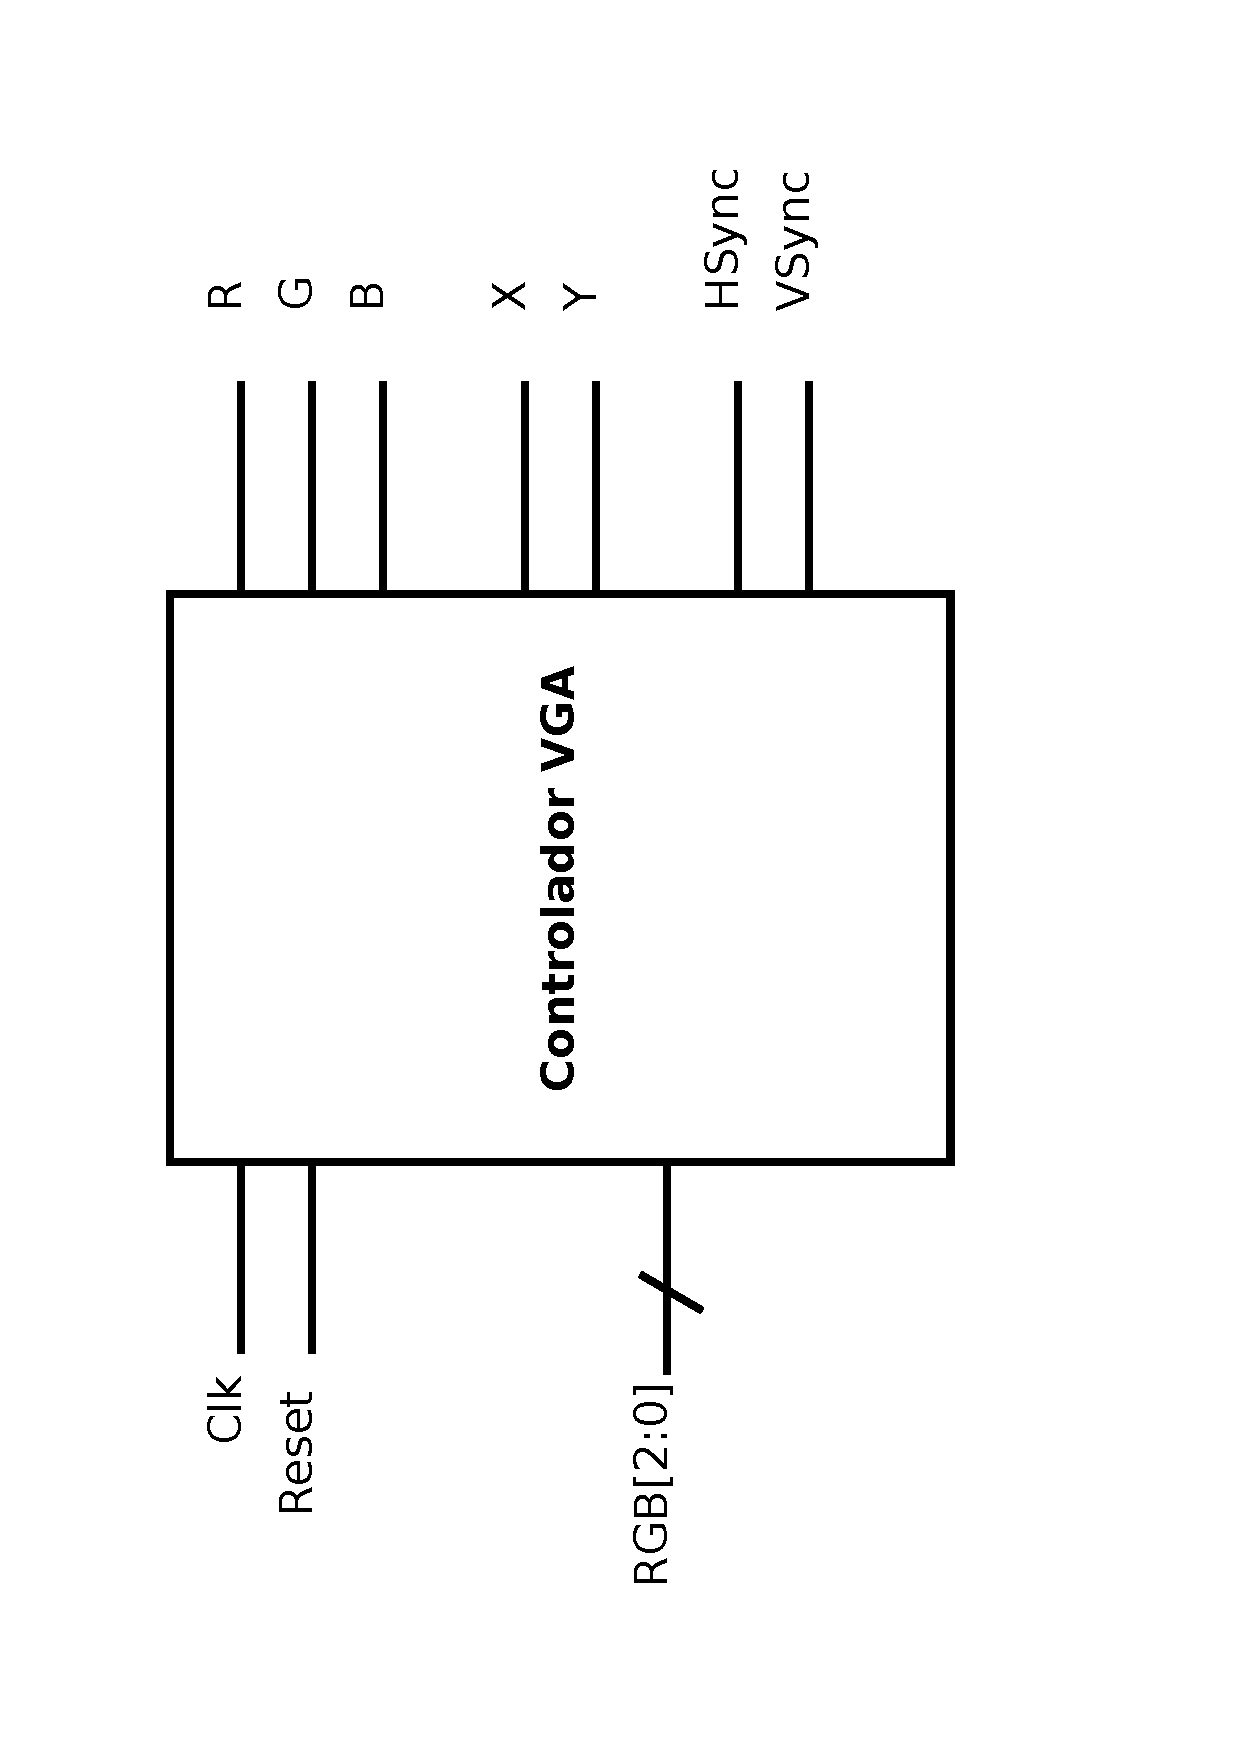
\includegraphics[width=0.4\textwidth, angle=-90] {vga_block.pdf}
	\caption{Diagrama de bloques del Controlador de pantalla VGA}\label{fig:vgaBlock}
\end{figure}

El controlador de pantalla VGA se encarga de generar el patrón de ondas necesario para mostrar los gráficos del juego en una pantalla externa.

El estándar VGA usa tres señales analógicas para codificar el color de cada píxel (R, G y B en la figura \ref{fig:vgaBlock}) y dos señales de sincronización que indican el fin de línea (HSync) y fin de pantalla (VSync). Para la implementación del controlador se ha usado una frecuencia de 25 MHz, que genera una resolución de 640 x 480 píxeles a una tasa de refresco de 60 Hz.

Para formar la imagen deseada en la pantalla, el controlador VGA accede a la información de color de cada píxel de manera similar a una memoria: las señales x e y indican la posición del píxel al bloque \hyperref[formatoVGA]{Formato VGA}, que devuelve el valor del color a través del bus \emph{RGB}. 

Dado que la placa de desarrollo \emph{Spartan 3E Starter Kit} contiene un conversor digital a analógico (DAC) de un sólo bit para las señales R,G y B, sólo es posible mostrar 8 colores diferentes en la pantalla.